\newpage


\section{Quadcopter Dynamics}

A quadcopter is a system of multibladed helicopter that is inherently unstable. It has a set of four rotors that are all coupled in both translational and rotational dynamics. The objective of these notes are to clearly derive governing equations of motion from first principles, and then to cast them in a way that is tractable and useful for the reader to be able to take and implement directly via simulation. 

\subsection{Free Body Diagram}

\begin{figure}[!h]
    \label{fig:quad}
    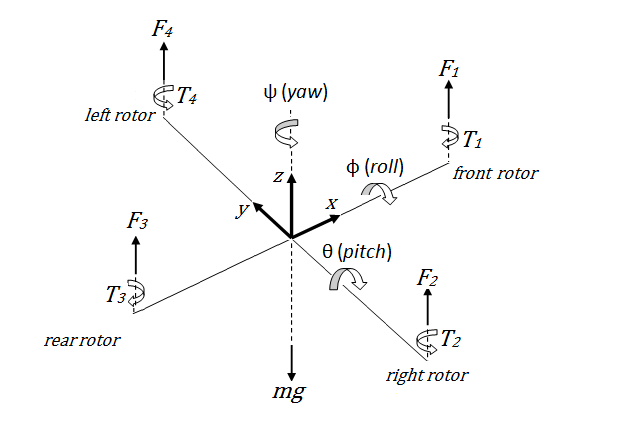
\includegraphics[width=.48\textwidth]{quadcopter}
\end{figure} 

\subsection{Governing Differential Equations of Motion}

\underline{\textbf{Inertial Frame Quantities:}}
$$\vect{P} = \bvecttrans{x}{y}{z} \quad \vect{V_{ref}} = \bvecttrans{\dot{x}}{\dot{y}}{\dot{z}}$$

\underline{\textbf{Body Frame Quantities:}}
$$ V_{body} = \bvecttrans{u}{v}{w} \quad , \omega^{body} = \bvecttrans{p}{q}{r}$$


$$\boxed{\bvectdot{u}{v}{w} = \frac{1}{m}\sum\vect{F} - \bvect{q w - r v}{r u -p w}{p v - q u}} $$

$$\boxed{ \bvectdot{p}{q}{r} = \bvect{\frac{\sum\tau_{1}}{I_{xx}}}{\frac{\sum\tau_{2}}{I_{yy}}}{\frac{\sum\tau_{3}}{I_{zz}}} - \bvect{\frac{(I_{zz} - I_{yy})}{I_{xx}}qr}{\frac{(I_{xx} - I_{zz})}{I_{yy}}pr}{\frac{(I_{yy}- I_{xx})}{I_{zz}}pq} \quad \quad \text{where} \quad \sum\vect{\tau} = \bvect{\sum\tau_{1}}{\sum\tau_{2}}{\sum\tau_{3}}}$$

$$\boxed{\sum F_{ext} \biggr\rvert_{body}= R_{zyx}(\phi, \theta, \psi)\biggr\rvert_{I}^{B}\left(\bvect{0}{0}{-mg} + \bvect{-k_d\dot{x}}{-k_d\dot{y}}{-k_d\dot{z}}\right) + k_{lift}\bvect{0}{0}{\sum\omega_{i}^{2}} }$$

$$\boxed{\tau_{body} = \bvect{\tau_{\phi}}{\tau_{\theta}}{\tau_{\psi}} = \bvect{Lk(\omega_{1}^{2} - \omega_{3}^{2})}{Lk(\omega_{2}^{2} - \omega_{4}^{2})}{b(\omega_{1}^{2}- \omega_{2}^{2} + \omega_{3}^{2} - \omega_{4}^{2})}}$$

$$ \bvect{p}{q}{r} = \begin{bmatrix}
    1 & 0 & -s(\theta)\\
    0 & c(\phi) & s(\phi)c(\theta)\\
    0 & -s(\phi) & c(\phi)c(\theta) \end{bmatrix}  \bvectdot{\phi}{\theta}{\psi}$$

$$ \bvectdot{\phi}{\theta}{\psi} = \begin{bmatrix}
    1 & s(\phi)t(\theta) & c(\phi)t(\theta)\\
    0 & c(\phi) & -s(\phi)\\
    0 & \frac{s(\phi)}{c(\theta)} & \frac{c(\phi)}{c(\theta)} \end{bmatrix} \bvect{p}{q}{r} $$
